\documentclass[a4paper, french, 12pt, titlepage]{article}
\usepackage[latin1, utf8]{inputenc}
\usepackage[T1]{fontenc}
\usepackage{graphicx,  amsmath, amssymb}
\renewcommand{\contentsname}{Sommaire}
\usepackage[margin = 1in]{geometry}
\graphicspath{{./images/}}


\title{Rapport de stage \\ Modélisation numérique d’oscillateurs non-linéaires pour
la récupération d’énergie vibratoire}
\author{LÉGLISE Cloé}

\begin{document}

\maketitle

\begin{center}
Je tiens à remercier Camille SAINT-MARTIN, ma tutrice de stage, pour m'avoir offert cette opportunité et m'avoir épaulée durant la totalité de ce stage.  \\
\end{center}

\begin{center}
Je souhaite également remercier Ludovic CHARLEUX, directeur de thèse de Camille SAINT-MARTIN, sans qui ce stage n'aurait pas été possible. \\
\end{center}

\begin{center}
Je suis aussi reconnaissante envers Abdourrahmane ATTO d'avoir pris du temps, en tant que tuteur école, de rechercher et m'envoyer des ressources, alors que ce n'était pas dans ses obligations. 
\end{center}

\newpage 

\tableofcontents

\newpage

\section*{Introduction}



PLAN 

\newpage 

\section{Contexte du stage}

\subsection{Présentation de l'organisme d'acueil}

L’Université Savoie Mont Blanc (USMB) est un établissement de 15 000 étudiants ouvert sur l’Europe et le monde. Les recherches sont menées par des laboratoires labellisés et reconnus, en partenariats étroits avec de grands organismes (CNRS, CEA, INRA), des organisations internationales (CERN) ou d’autres structures (INES, ”Institut de la Montagne”) à la pointe de l’innovation. Le SYMME (”Systèmes et Matériaux pour la Mécatronique”) est l’un de ces laboratoires. Il a été créé en 2006 pour renforcer la position stratégique de l’université dans le domaine de la mécatronique. Il emploie environ 80 chercheurs, personnel administratif et étudiants. Ses recherches dans le domaine des microsources d’énergie concernent notamment le développement de structures électromécaniques innovantes aux échelles centimétrique et millimétrique, capables de convertir des énergies mécaniques en énergie électrique. Ces travaux recouvrent les aspects mécaniques et électroniques dans une approche multiphysique globale et cohérente. Plus particulièrement, ses activités de recherche portent sur les transducteurs piézoélectriques, électromagnétiques et électrostatiques pour la conversion d’énergie, sur des oscillateurs mécaniques linéaires et non-linéaires pour élargir la bande de fréquence des générateurs, et sur des interfaces électriques pour le conditionnement de l’énergie et le suivi de fréquences. Ses travaux ont fait l’objet de nombreuses communications dans des journaux et des conférences de référence dans le domaine et sont reconnus par la communauté scientifique.\\


Les travaux au laboratoire SYMME suivent deux axes principaux : "Matériaux, Systèmes et Instrumentation Intelligents", et "Qualité Industrielle". Ces deux thèmes sont eux-mêmes divisés en trois thèmes chacuns, respectivement : "Matériaux et nanomatériaux fonctionnels", "Instrumentation pour le médical", et "Valorisation de micro-sources d'énergies ambiantes" ; et "Caraxtérisation et modélisation thermomécanique des matériaux", "Optimisation produit-procédé" et "Optimisation des processus". \\

\begin{figure}
  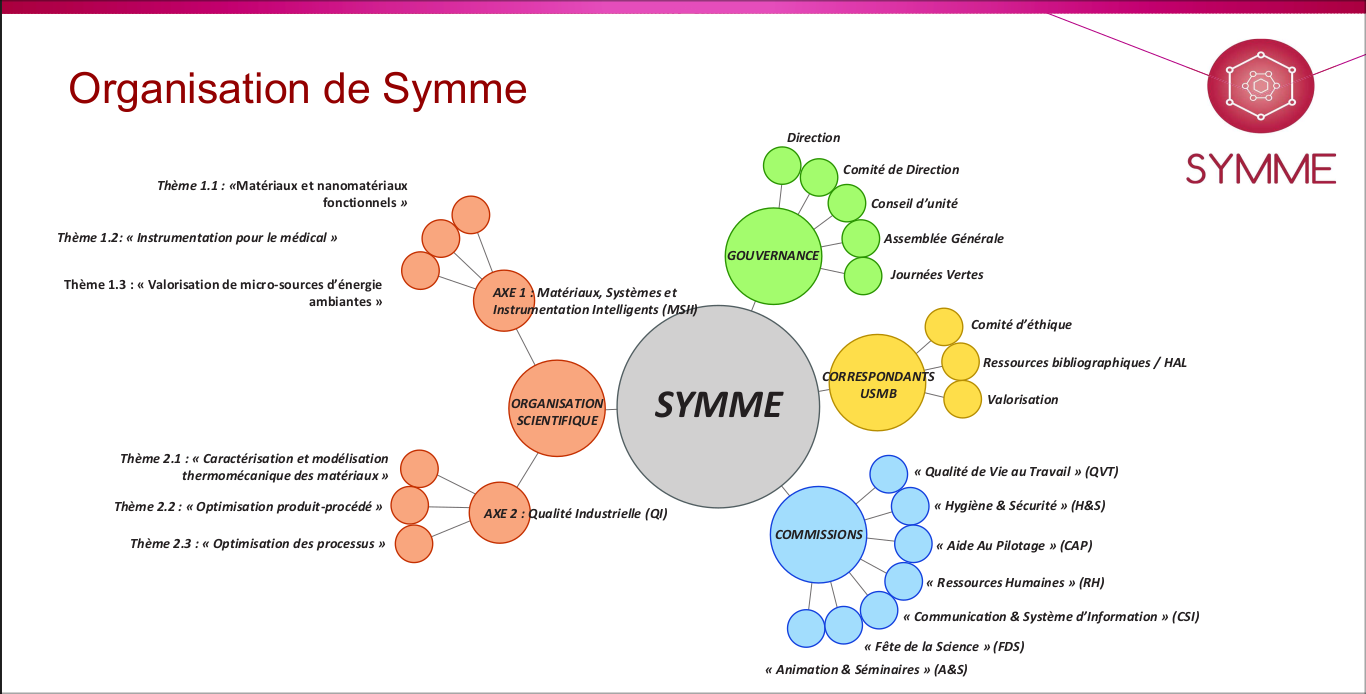
\includegraphics[width=\linewidth]{organigramme.png}
  \caption{Organisation du laboratoire SYMME}
  \label{fig:organigramme}
\end{figure}
La figure 1 montre l'organisation du laboratoire SYMME. 

C'est dans le thème "Matériaux, systèmes et instrumentation intelligents - valorisation de micro-sources d'énergies ambiantes" que s'inscrit ce stage. 

\subsection{Sujet de stage}

Le déploiement de réseaux de capteurs sans fil communicants nécessite l’utilisation de batteries qui ont une durée de vie limitée. Le domaine de la récupération d’énergie vibratoire vise à remplacer, ou du moins complémenter, l’usage de ces batteries au moyen de systèmes innovants de récupération et de stockage d’énergie robustes et fiables. Un récupérateur d’énergie vibratoire est généralement composé d’un oscillateur mécanique, de transducteurs électromécaniques (par exemple des transducteurs piézoélectriques) pour la conversion de l’énergie mécanique des vibrations en énergie électrique et d’un circuit d’extraction électrique. Les premiers travaux dans le domaine utilisaient des récupérateurs linéaires, c’est-à-dire, ceux composés d’un oscillateur linéaire. Cependant, de tels récupérateurs présentent une bande de fréquences étroite et ne sont donc pas adaptés à un environnement présentant un spectre de vibration riche et varié. Une solution prometteuse pour élargir la bande de fréquences est de considérer un oscillateur non-linéaire. Cependant, les comportements des récupérateurs non-linéaires sont plus difficiles à prédire de part l’existence de plusieurs solutions pour une fréquence de vibration donnée. Une analyse approfondie est nécessaire pour une compréhension complète de la dynamique. Dans le cadre du stage, le candidat sera en charge de modéliser un récupérateur non-linéaire développé au sein du laboratoire SYMME et se familiarisera avec les outils numériques déjà mis en place.

L’objectif de ce stage est de développer une interface graphique pour l'analyse d'influence des paramètres du modèle. La dynamique pourra être visualisée sur l’interface. Le projet open-source sera développé en Python ou en Julia. Le stagiaire définira les fonctionnalités de l’application et passera à la phase de développement de l’application. Par exemple, il faudra faire en sorte que l’utilisateur puisse choisir un modèle de récupérateur d’énergie vibratoire, définir le type d’excitation, changer les valeurs numériques des paramètres et choisir les variables qu’il souhaite visualiser. Le stagiaire utilisera un outil de développement logiciel open-source de son choix (Gitlab, GitHub) afin d’assurer une intégration continue et associer une documentation (manuel d’utilisation) à l’application. Durant le stage, le candidat développera ses compétences en développement logiciel et modélisation numérique. Il sera intégré dans une équipe ayant une expertise dans la modélisation, conception et développement de solutions pour la récupération d’énergie, au laboratoire SYMME (Annecy). Selon l’avancement du stage, l’application développée par le stagiaire pourra faire l’objet d’une publication d’un article scientifique.

\newpage

\section{Contexte scientifique}


\subsection{Les récupérateurs d'énergie}

L'utilisation de récupérateurs d'énergie permet de récolter de l'énergie vibratoire. Il en existe de plusieurs sortes, par exemple les récupérateurs d'énergie piézoélectriques linéaires, qui peuvent amplifier les vibrations s'ils sont excités à leur fréquence naturelle. Ceci dit, ces récupérateurs d'énergie ne peuvent récupérer une puissance importante qu'au sein d'une bande passante très étroite. Les récupérateurs d'énergie vibratoire non linéaires ont une bande passante bien plus large, bien que la complexité de leurs comportement peuvent les rendre difficiles à analyser. 

Les récupérateurs d'énergie non linéaires multi-stables peuvent présenter plusieurs cycles limites stables, appelés orbites, qui dépendent des conditions initiales. Certaines de ces orbites, appelées orbites hautes, correspondent à un mouvement oscillatoire entre deux positions stables de la masse inertielle. D'autres, appelées orbites basses, correspondent à une situation à la masse inertielle oscille faiblement autour d'une seule position stable. Les orbites hautes sont beaucoup plus intéressantes pour la récupération d'énergie, parce qu'elles représentent une puissance plus importante. Il est donc intéressant de mettre en place des stratégies de saut d'orbites, permettant à l'oscillateur de passer d'une orbite faible à une orbite basse. 

Pour effectuer un saut d'orbite, il faut nécessairement donner de l'énergie à l'oscillateur. Il faut donc trouver une méthode la moins coûteuse en énergie possible pour que la manipulation soit rentable. Pour un oscillateur bistable de Duffing, cinq paramètres jouent un rôle important dans son comportement : la masse M, la raideur k, la valeur des positions stables $x_0$, la longueur L et l'amortissement µ. Notons que le niveau de flambement, donné par $\frac{x_0}{L}$, sera indirectement modifié par la modification d'autres paramètres. Ainsi, en touchant l'un de ces paramètres, on peut augmenter l'énergie potentielle du système et ainsi le faire passer d'une orbite basse à une orbite haute. 


\subsection{Cahier des charges}

\newpage 

\section{Contenu du stage}


\subsection{Travail effectué}


Durant ce stage, différents outils de travail ont été utilisés. La totalité du code écrit se situe dans un repository Git, dont l'utulisation a permis de travailler en équipe, récupérer d'anciennes versions du code, et l'application finale disponible. La programmation a été réalisée sur l'éditeur de code Visual Studio Code, dont les nombreuses extensions permettent d'utiliser de nombreux langages différents, ainsi que des outils tels que Git de manière rapide et instinctive. Après plusieurs discussions, il a été décidé que la programmation serait faite en utilisant le langage Julia, plus rapide et performant que Python, et avec des librairies simplifiées sur la résolution d'équations différentielles et l'affichage de graphes interactifs. \\

Travailler sur ce sujet a impliqué d'essayer différentes librairies Julia afin de mieux se rendre compte de ce qu'il était possible de faire avec ce langage. Il a vite été important de savoir exactement ce que les outils intégrés à Julia permettent de réaliser comme interface graphique. Pour cela, la modélisation des oscillateurs a d'abord été faite "à la main", en suivant une résolution d'équation différentielle numérique à l'aide de la méthode de Runge-Kutta d'ordre 4. Il s'est ensuite avéré que plusieurs paquetages Julia étaient capables de faire cette résolution de manière beaucoup plus rapide et intégrée dans différentes fonctions d'animation. Il existe, en Julia, une librairie de systèmes dynamiques déjà enregistrés. Il est possible de créer son propre système dynamique avec les équations qui le caractérisent afin qu'il se comporte de la même manière que ceux qui ont été pré-enregistrés, ce qui est très utiles car certaines fonctions d'animations interéssantes ne fonctionne qu'avec un système dynamique en entrée. Un oscillateur bistable a donc été codé de cette manière, déclaré comme système dynamique afin de se servir de ces propriétés. Mais la modélisation initiale a servi pour faire différents essais d'interface graphique. \\


\subsubsection{Interface graphique}

Il est vite devenu apparent que le paquetage Gtk.jl permettait de créer des interfaces graphiques interactives assez facilement. La création de curseurs pour modifier les paramètres et de menus déroulants pour changer de conditions initiales a été étudiée afin de faire une fenêtre permettant de modifier un graphique. Les graphiques ont été codés à l'aide de du paquetage Plots.jl. L'utilisation de macros, qui viennent du langage Lisp, permettent de créer de GIFs ou des animations en seulement une ligne de code. Ces différentes fonctionnalités ont été utilisées pour réaliser une première fenêtre interactive. Cette première fenêtre simule la trajectoire d'un oscillateur répondant à l'équation $\ddot x = - \delta * \dot x - \alpha * x - \beta * x^3 + t $ de deux manières: à gauche, un graphe statique, et à gauche un gif dynamique du même graphe. Sur le graphe de gauche, le tracé bleu représente exactement la même trajectoire que sur le gaphe de droit, et le tracé orangé représente un oscillateur avec les mêmes paramètres, maisdont les conditions initiales peuvent être définies par le menu déroulant juste au-dessus, sur la droite de la fenêtre. À gauche de ce menu déroulant se trouvent trois curseurs correspondant respectivement aux paramètres $\alpha$, $\beta$ et $\delta$. \\

La figure 2 est une vue classique de cette fenêtre, c'est ce que l'utilisateur peut voir à l'exécution du code.\\

\begin{figure}[htb]
  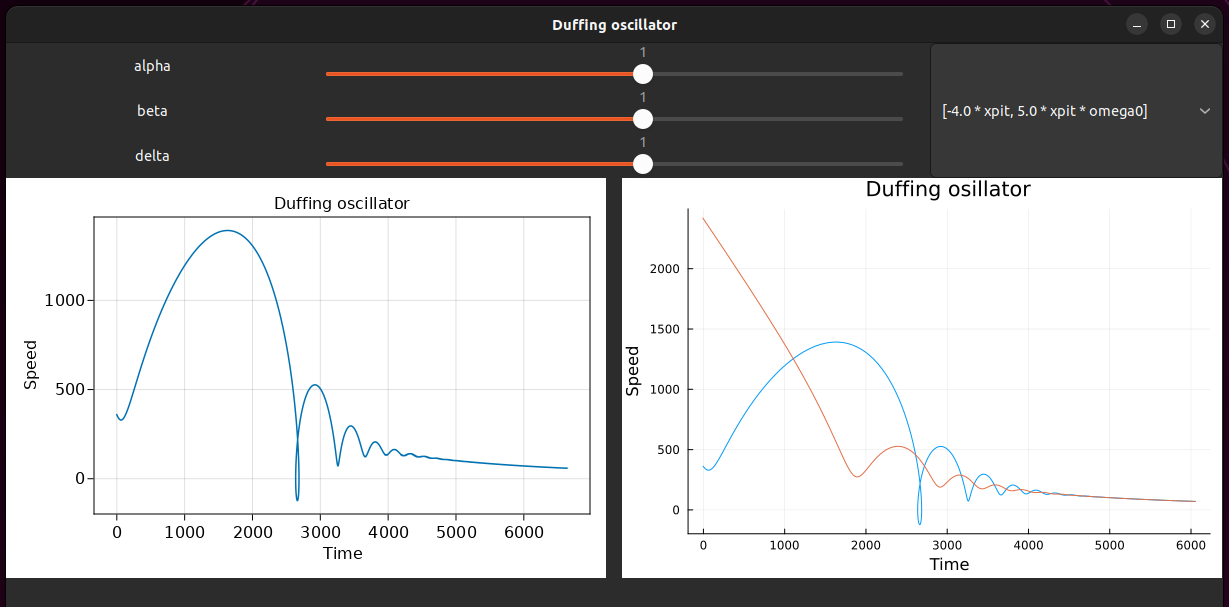
\includegraphics[width=\linewidth]{interactivewindow_1.png}
  \caption{Vue classique de la fenêtre interactive créée avec le paquetage Gtk.jl}
  \label{fig:organigramme}
\end{figure}

La figure 3 permet d'illustrer le mouvement du graphe de droit : la capture a été prise à un moment où le graphe n'est pas encore complet. Ce graphe se crée en boucle : une fois arrivé à la fin du temps pris pour la trajectoire, il s'efface et recommence. \\

\begin{figure}[htb]
  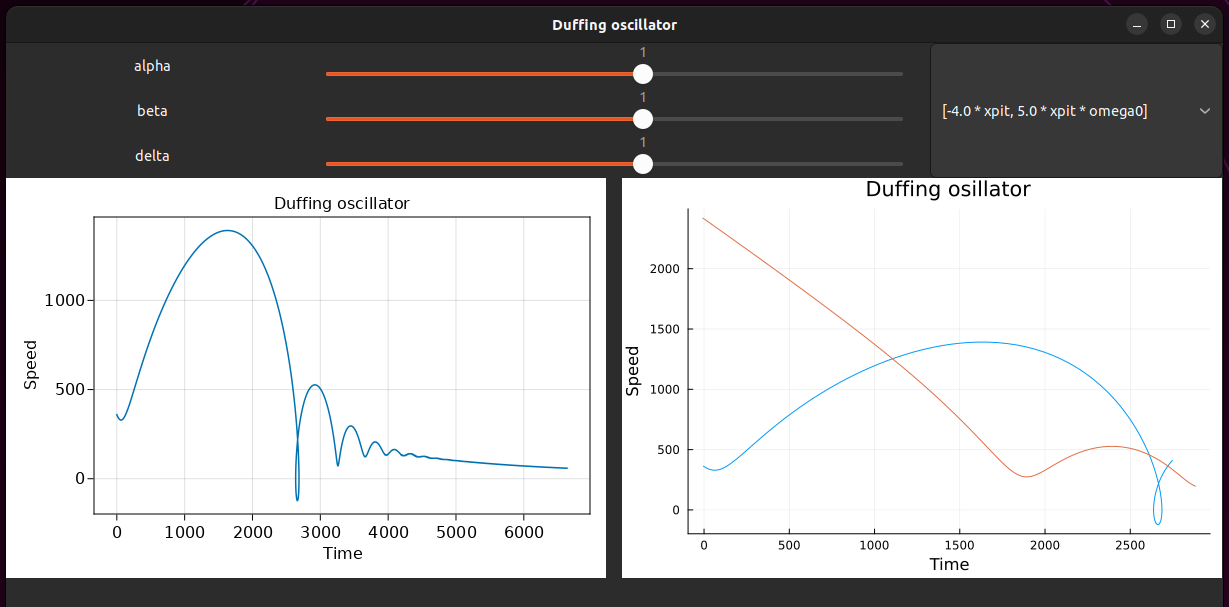
\includegraphics[width=\linewidth]{interactivewindow_2.png}
  \caption{Vue de la fenêtre interactive avec le gif pris à un autre moment}
  \label{fig:organigramme}
\end{figure}

Les curseurs permettent de modifier les paramètres de l'équation différentielle et voir leur impact immédiatement sur les graphes. La figure 4 donne une vue de la fenêtre interactive avec l'un des paramètres modifiés. \\

\begin{figure}[htb]
  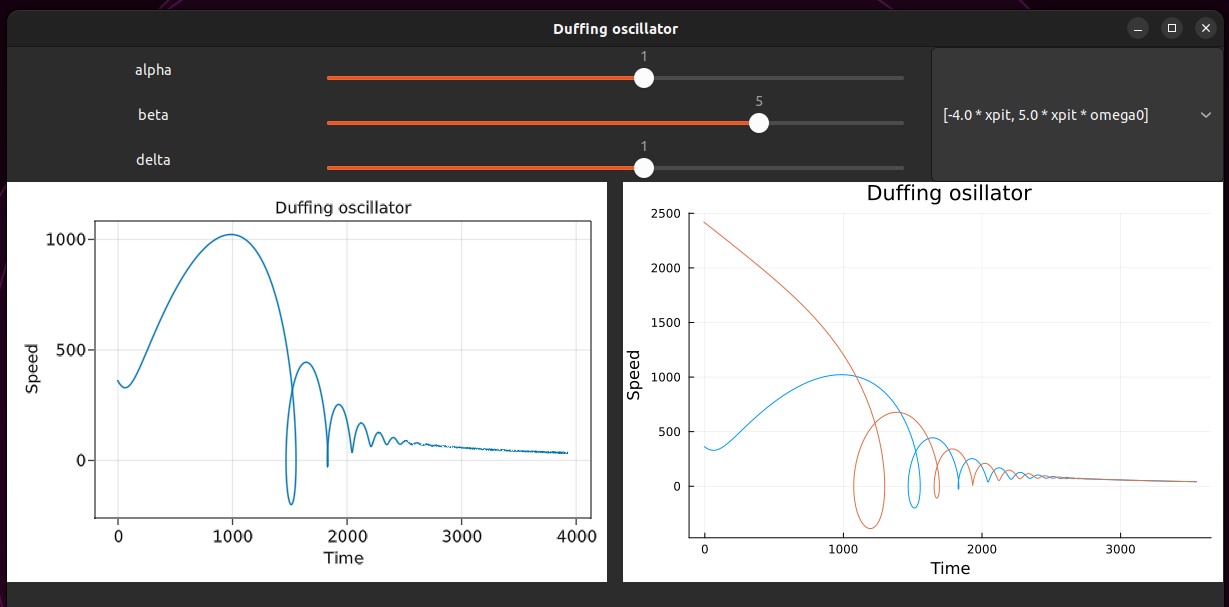
\includegraphics[width=\linewidth]{interactivewindow_3.png}
  \caption{Vue de la fenêtre interactive avec des paramètres différents}
  \label{fig:organigramme}
\end{figure}

Le menu déroulant en haut à droite de la fenêtre permet de modifier les conditions initiales du tracé orange sur le graphe de droite. La figure 5 montre ce qu'une modification de ces conditions initiales donne. \\

\begin{figure}[htb]
  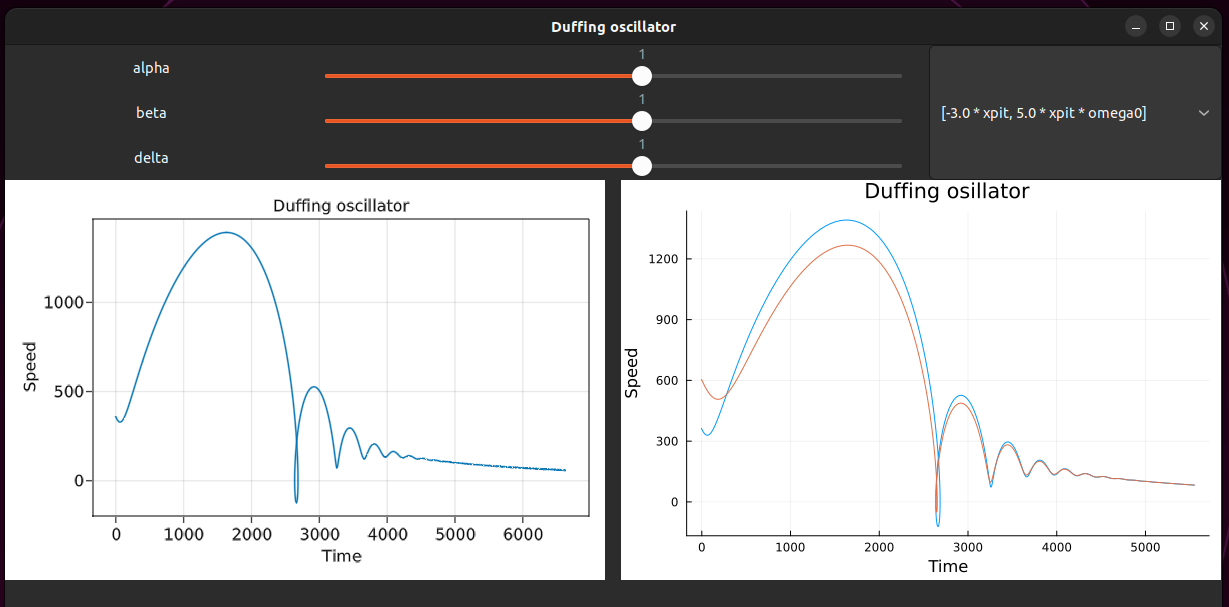
\includegraphics[width=\linewidth]{interactivewindow_4.png}
  \caption{Modification des conditions initiales pour le tracé orange}
  \label{fig:organigramme}
\end{figure}


Une autre façon de créer des interfaces graphiques en Julia est d'utiliser l'extension Visual Studio Code Génie Builder. Cette extension permet d'organiser une fenêtre graphique avec un système de "cliqué-glissé" qui se construit automatiquement en générant un code html. Il est ainsi possible de mettre en place tous les éléments souhaités (graphes, boutons, curseus, menus déroulants... mais aussi textes interactifs, par exemple) de manière intuitive et rapide. À condition de maîtriser l'outil, cela peut permettre de gagner beaucoup de temps pour le côté purement graphique de l'application. Un fichier app.jl contient le code de l'application en elle-même, c'est-à-dire le code des modélisations, calculs et autres programmations nécessaires. Il faut ensuite créer des variables spécifiques contenant, par exemple, le résultat d'un calcul. Ces variables-là communiquent avec l'interface. Dans l'onglet qui sert à créer l'interface par système de cliqué-glissé, il suffit de sélectionner un élément mis en place afin d'en modifier certaines caractéristiques, notamment quelles sont les valeurs ou actions qui lui sont associées. \\

La figure 6 montre la fenêtre de travail de l'extension Génie Builder. C'est une fenêtre générée automatiquement lors de la création d'une nouvelle application. Sur la droite, sous la catégorie "Bindings", se trouvent toutes les variables permettant de communiquer entre l'interface et le code du fichier app.jl. Sur l'interface de travail, le graphique (dernier élément, en bas) est sélectionné. Dans la colonne de droite, il est possiblie d'en modifier les propriétés, par exemple les valeurs prises dans le champ "Data". \\

\begin{figure}[htb]
  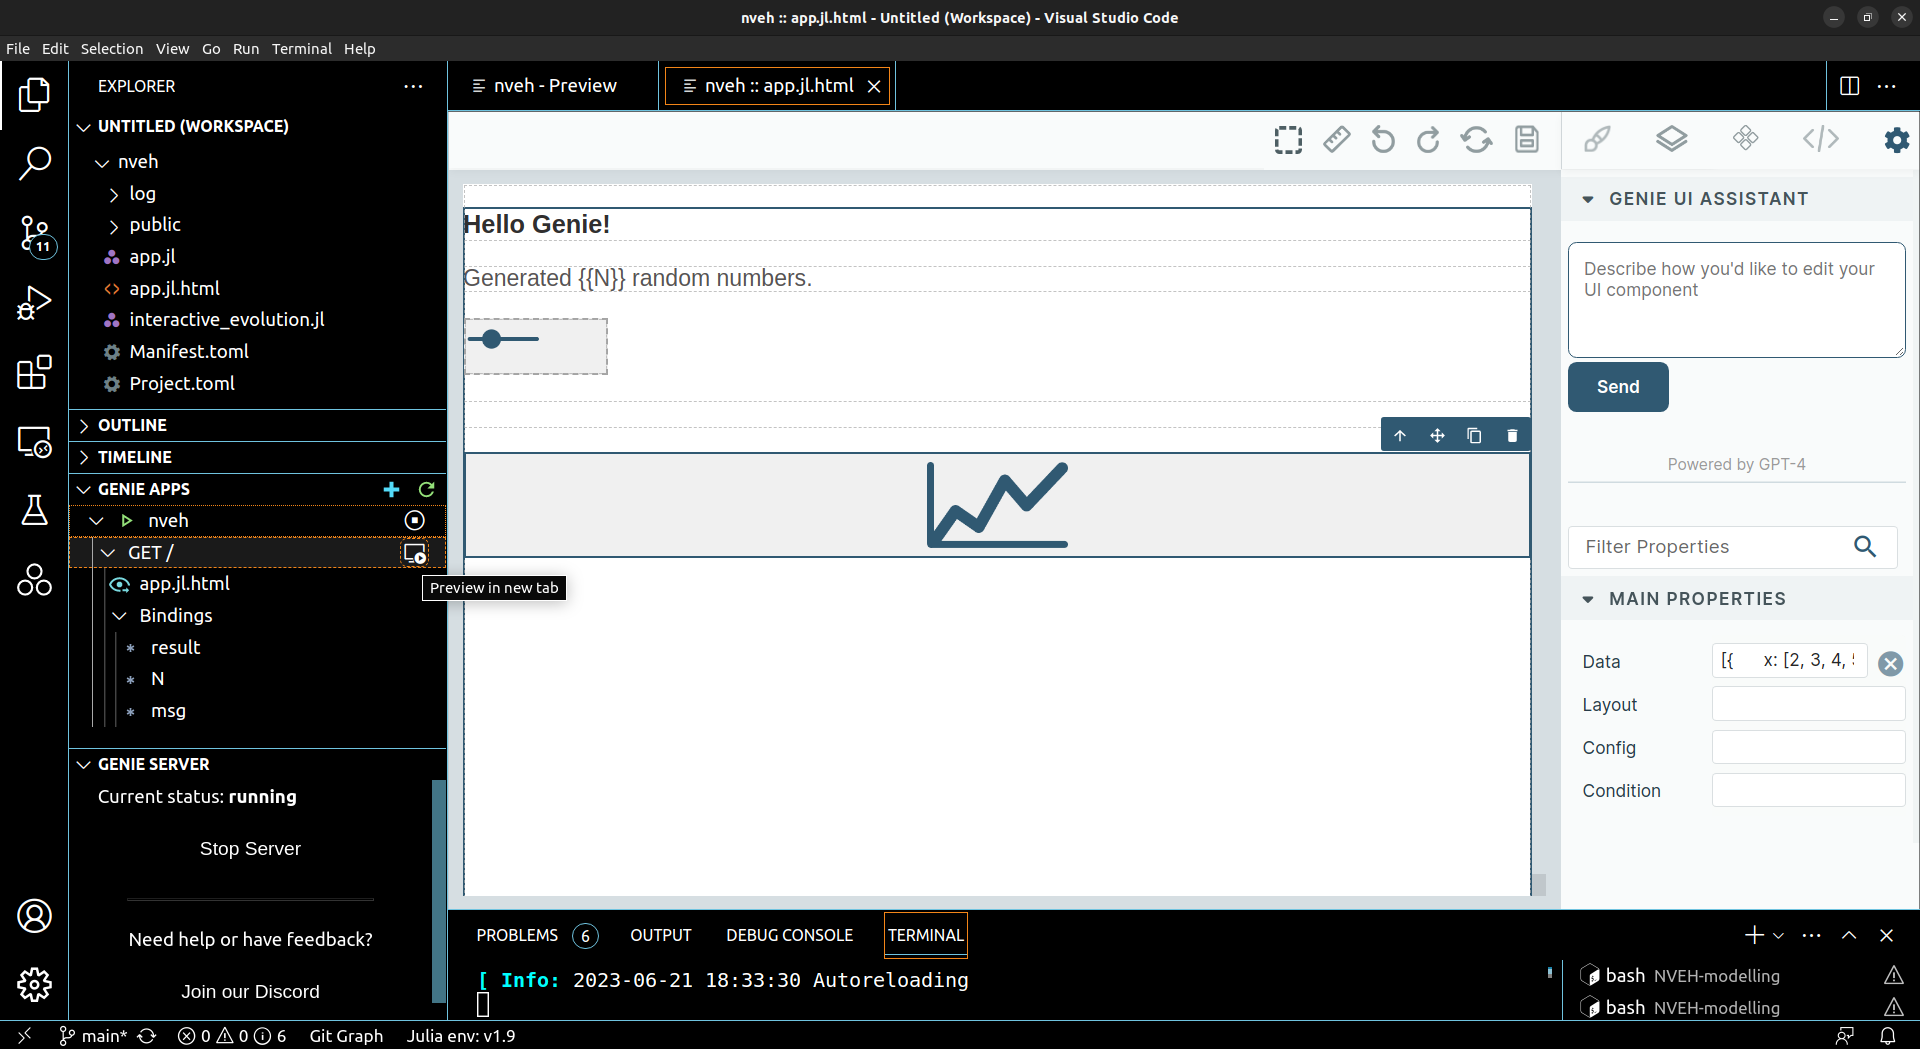
\includegraphics[width=\linewidth]{geniebuilder_travail.png}
  \caption{Fenêtre de travail de Génie Builder}
  \label{fig:organigramme}
\end{figure}

La figure 7 montre l'aperçu de la fenêtre générée par le code de la figure 6. Le curseur, interacif, et les deux messages qui se modifient lorsque le curseur est bougé, y sont présents, ainsi que le graphe avec les valeurs vues plus haut. \\

\begin{figure}[htb]
  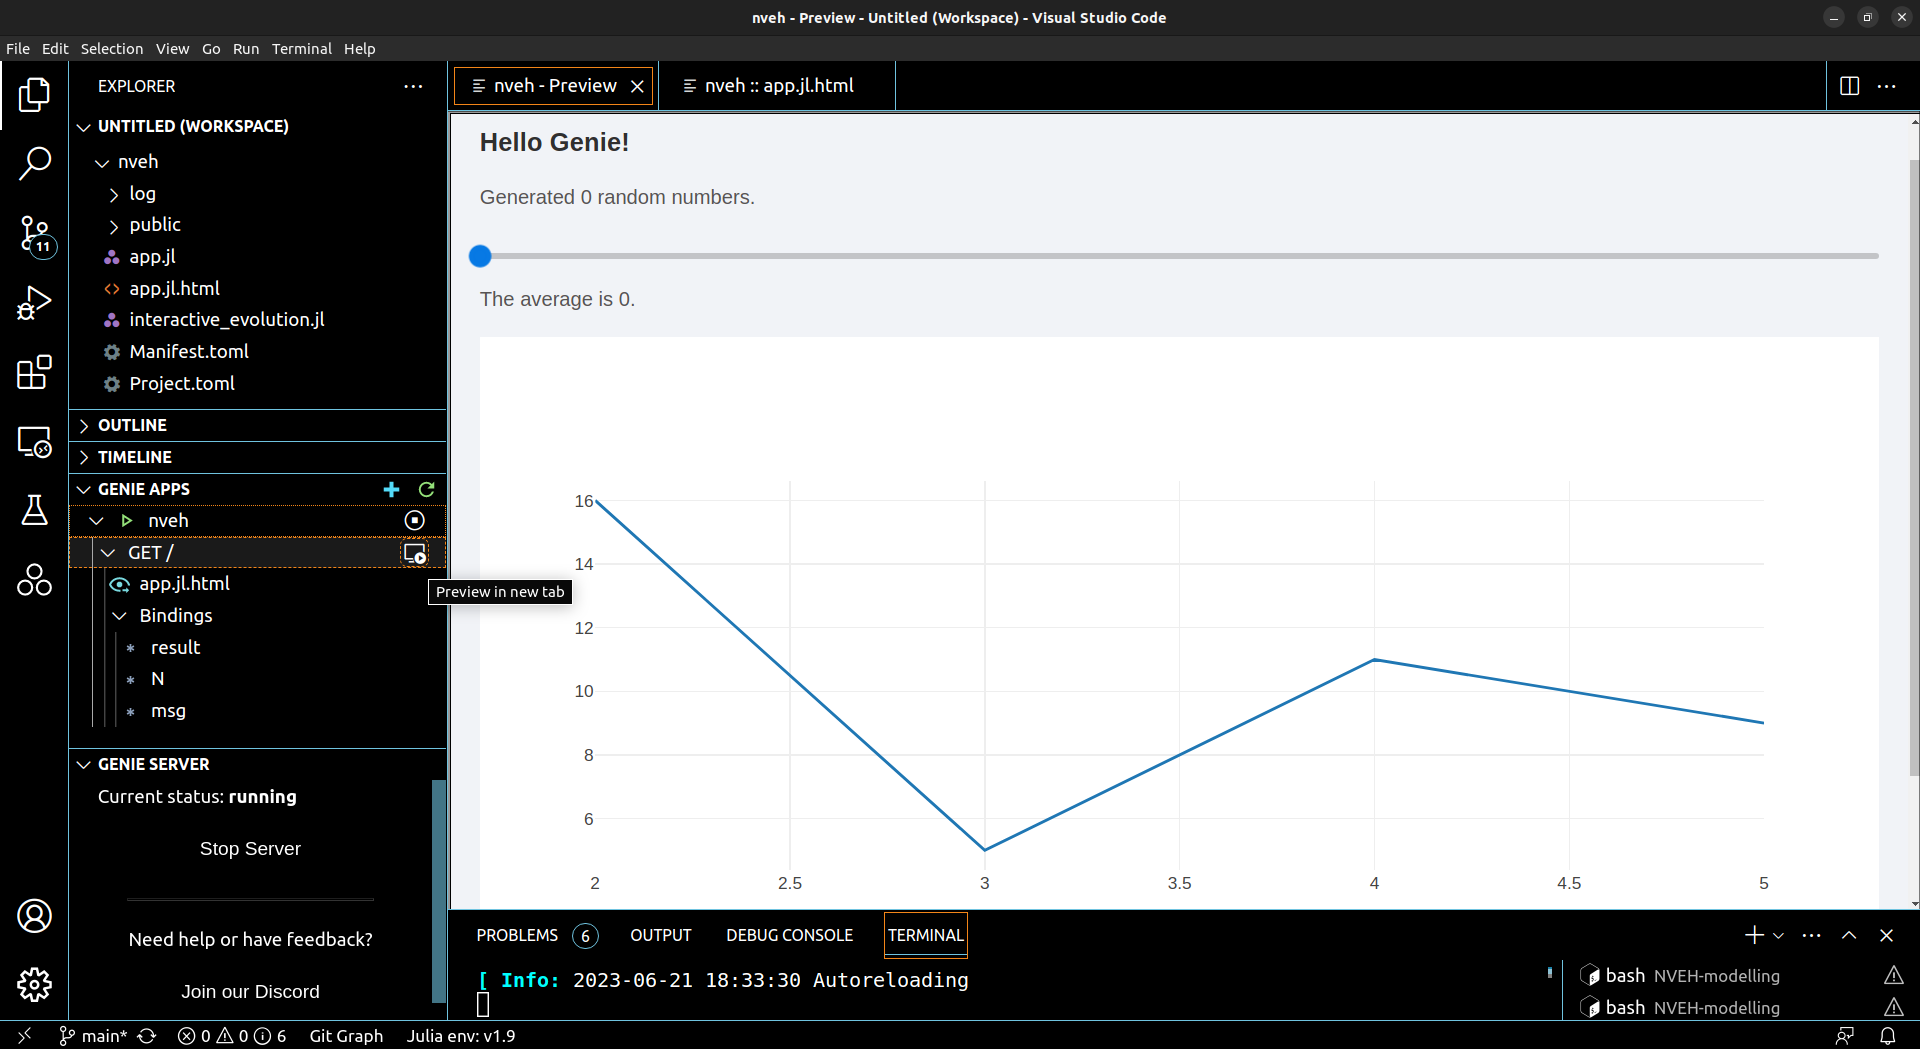
\includegraphics[width=\linewidth]{geniebuilder_result.png}
  \caption{Aperçu du résultat de Génie Builder}
  \label{fig:organigramme}
\end{figure}


Ce système a été retenu comme une possibilité pour créer l'application finale car, si maîtrisé correctement, il pourrait permettre de prendre beaucoup moins de temps sur le côté esthétique pour agencer correctement l'interface, et permettre de se concentrer un peu plus le côté modélisation et programmation.  \\


\subsubsection{Système dynamique}

En Julia, il existe de nombreux paquetages permettant de manipuler des systèmes dynamiques de manière simplifiée. Le premier qui sera abordé ici est le paquetage \emph{HarmonicBalance.jl}. Ce paquetage utilise la méthode de la balance harmonique pour calculer des solutions périodiques en passant par le domaine fréquentiel. Ainsi, par exemple, pour un oscillateur répondant à l'équation $\ddot x(t) + \omega_0^2 x(t) + \alpha x(t)^3 + \eta x(t)^2 \dot x (t) = F \cos(\omega t)$ le calcul et l'affichage des solutions réelles donne le graphe vu en figure 8. \\

\begin{center}
\begin{figure}[htb]
  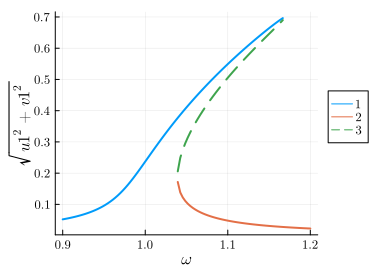
\includegraphics[width=0.7\linewidth]{harmonicbalance.png}
  \caption{Aperçu du résultat de Génie Builder}
  \label{fig:organigramme}
\end{figure}

\end{center}

\subsection{Ce qu'il reste à faire}

\newpage 

\section*{Conclusion}


\newpage 

\section*{Bibliographie}

Saint-Martin, C., Morel, A., Charleux, L., Roux, E., Benhemou, A., \& Badel, A. (2022). Power expectation as a unified metric for the evaluation of vibration energy harvesters. Mechanical Systems and Signal Processing, 181, 109482.\\

Huguet, T. (2018). Vers une meilleure exploitation des dispositifs de récupération d’énergie vibratoire bistables: Analyse et utilisation de comportements originaux pour améliorer la bande passante (Doctoral dissertation, Université de Lyon).\\

Liu, W. (2014). Conception d'un dispositif de récupération d'énergie vibratoire large bande (Doctoral dissertation, Grenoble).\\


@article{10.21468/SciPostPhysCodeb.6,
	title={{HarmonicBalance.jl: A Julia suite for nonlinear dynamics using harmonic  balance}},
	author={Jan Košata and Javier del Pino and Toni L. Heugel and Oded Zilberberg},
	journal={SciPost Phys. Codebases},
	pages={6},
	year={2022},
	doi={10.21468/SciPostPhysCodeb.6},
	url={https://scipost.org/10.21468/SciPostPhysCodeb.6},
}

	
\end{document}

